\chapter{Literature Review}
\label{chp:LR}

%%%%%%%%%%%%%%%%%%%%%%%%%%%%%%%%%%%%%%%%%%%%%%%%%%%%%%%%%%%%%%%%%%%%%%%
\section{Soft Robotics}

The field of soft robotics comprises robots and robotic actuators constructed from compliant and pliable materials, or exhibiting compliant behaviour \cite{Wang2015, Ilievski2011}. Hyper-elastic materials are often used in the construction of soft robots.

Soft

Soft robots generally have fixed joints and locomotive actuators between joints, as opposed to traditional hard robots which usually have locomotive actuated joints connected by rigid sections \cite{Whitesides2018}, as illustrated in Figure~\ref{fig:rad}.

\begin{figure}
	\begin{subfigure}[b]{0.4\textwidth}
		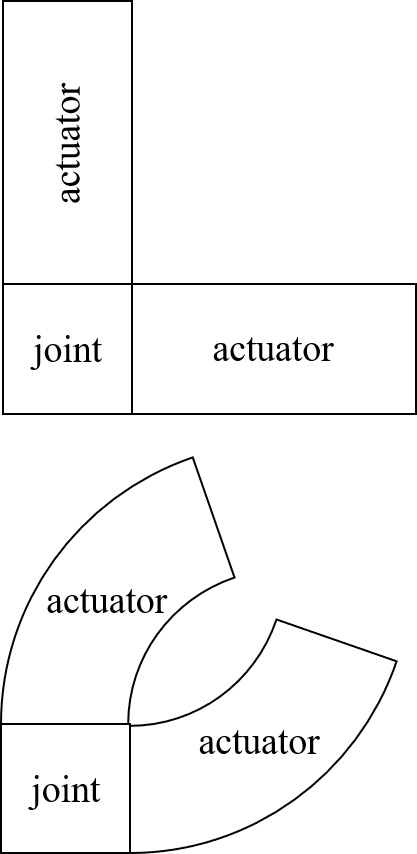
\includegraphics[width=\textwidth]{SR_JA.png}
		\caption{Soft Robot Actuation}
	\end{subfigure}
	\hfill
	\begin{subfigure}[b]{0.4\textwidth}
		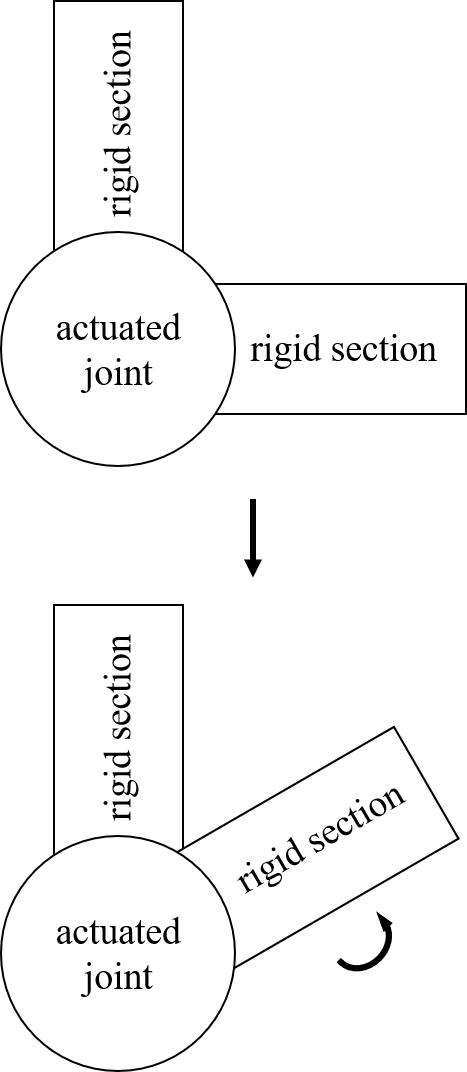
\includegraphics[width=\textwidth]{TR_JA.png}
		\caption{Traditional Robot Actuation}
	\end{subfigure}
	\caption{Robot Actuation Differences}
	\label{fig:rad}
\end{figure} 

Soft robots offer many advantages over traditional robots. Soft robots are safer in working environments alongside humans. Traditional robots are generally comprised of non-compliant hard materials such as steel or aluminium. These materials are often dense and heavy. Traditional robots usually have fixed motion paths and do not deviate easily. Humans working alongside traditional robots may easily be injured by these robots if they are struck or trapped by them. Soft robots are built with compliant and lightweight materials. Soft robots also generally exert lower forces than their traditional counterparts \cite{Martinez2013}.

Soft robots are more suited to working with fragile and irregular objects such as fruit. In addition to the reasons listed above, soft robots easily adjust to deviations when deforming \cite{Martinez2013, Whitesides2018}.


New soft robot developments



\section{Actuators}

Actuators are components that cause controlled motion, generally used in robotics and machinery \cite{Sekhar2012}. There are currently a few major types of soft robotic actuators in use \cite{Boyraz2018}.

\subsection{Actuator Types}

Shape Memory Alloys (SMA) are metallic alloys capable of being formed into a specific shape while above an inherent transformation temperature, as well as being formed into another shape below the transformation temperature. When the material is then heated or cooled above or below the transformation temperature, it reforms into those respective shapes. This property exists due to the transition between the martensite phase of the material below the transformation temperature, and the austenite phase above the transformation temperature. SMA actuators are heated by applying a current directly to the material. SMA actuators are small, lightweight, silent, and have a high force-to-weight ratio. When shaped straight, they can exert high forces, but only achieve small displacements relative to their length. When coiled, they can extend more, but exert smaller forces. \cite{Villoslada2015}

Shape Memory Polymers (SMP) are similar to SMAs, consisting of smart polymers with the same shape memory properties, instead of metallic alloys. The initial is shape is determined during the manufacturing process. The transformed shape is obtained by cooling the SMP and shaping it as desired. SMPs use electricity or light as a heat source for transformation \cite{Behl2007}. They have a high deformation capacity and shape recovery. They are lighter, cheaper and easier to produce than SMAs. They are limited in size due to their low recovery stresses \cite{Rodriguez2016, Behl2007}.

Dieelectric/Electrically-Actuated Polymers (DEAP) consist of layers of polymers interspersed with conductive material. When the conductive material receives an electrical input, a chemical reaction occurs that causes a change in volume across the layers. This causes the layers to bend in a predetermined direction. DEAPs are lightweight, silent and use little energy. They are biocompatible and functional in water. They are well-suited to mimicking real muscles. Their reactions under high voltages are not fully understood yet and accurately modelling them is highly complicated. \cite{Mutlu2014}

Electro-Magnetic Actuators (EMA) make use of magnetic microparticles within a polymer matrix. The particles are manipulated to cause motion by an external magnetic field from an electromagnet. This allows for a wide range of motion by varying the orientation and magnitude of the electromagnetic field. EMAs are small, require low voltages and are efficient. They have quick response times and high dynamic ranges. They are still an emerging technology in the early stages of development. \cite{Do2018}

Fluid Elastomeric Actuators (FEA) use soft polymeric structures with internal geometry designed for specific types of motion when driven by fluid pressure. Fluid pressure may be obtained from pressurized containers or chemical reactions. They are simple to design, manufacture and control, and are lightweight and usually inexpensive. They are scalable to different sizes and resistant to many types of damage. \cite{Shepherd2011,Onal2017}

\subsection{Actuator Shapes}

Multiple types of soft robotic actuators implement linear extension. This allows for an increase in reach and activation of levers or switches. Torsional extension is a variant of linear extension. Torsionally extending actuators twist as they extend, resulting in an angular difference between the ends of the actuator. \cite{Whitesides2018}

FEAs can be built to curl while contracting and straighten out while expanding, similar to natural muscles. This has a range of applications, especially when multiple of these FEAs are used in conjunction with one another. One application is as a gripper, where a number of these FEAs are arranged similarly to a hand or tentacles all curling inward. Grippers are well-suited to picking up and manipulating soft and/or irregularly shaped objects. \cite{Whitesides2018}

Non-trivial actuators are manufacturable. A bimodal FEA was developed by Ellis in 2020. The actuator has a crimped paper strip acting as a strain limiter embedded within a stiff layer of Ecoflex 0030. The stiff layer is alongside multiple Mold-Star 15 cells. When pressurised by a linearly increasing single pressure source, the actuator  first curls inwards, then back outwards while extending linearly. \cite{Ellis2020}

%%%%%%%%%%%%%%%%%%%%%%%%%%%%%%%%%%%%%%%%%%%%%%%%%%%%%%%%%%%%%%%%%%%%%%%
\section{Soft Robot Modeling}

To prevent having to physically construct every design of a soft body, a computationally efficient and accurate digital model can be constructed.

\subsection{Modeling Approaches}

The Finite Element Method (FEM) is an approach to numerically solving field problems. Field problems require the determination of one or more dependent variables' distribution in space. Field problems are mathematically described with differential equations or integral expressions. Finite elements can be expressed as small parts of a larger body. A field quantity within an element may only have a simple spatial variation, such as being described by polynomial terms no higher than the second order. FEM differs from calculus as calculus uses infinitesimal elements. FEM thus delivers approximate solutions. \cite{Cook2002}

Voxels are three dimensional (3D) pixels. Voxels are usually cubical. Realistic physical properties may be applied to voxels in specific software packages, such as the free VoxCAD software. Bodies may be constructed and undergo deformation when constructed from voxels in these software packages. It is relatively simple to construct bodies from voxels. \cite{Cheney2013,Cheney2015}

The Gaussian Mixtures representation uses a density field analogy to a level-set method. The density field is initialised as having zero density. Points of density with Gaussian falloff are added within the field. The points may have positive or negative weights. Positive weights contribute to the density, while negative weights subtract from it. If a single point was used, a solid sphere would be the thresholded result. 

\subsection{Modeling Software}

Several commercial software packages capable of realistically modeling soft bodies are available.

LSDyna is a FEM software package widely used in industry. It is owned by ANSYS and maintained by LST. The software's code is based on highly non-linear and transient dynamic FEM with explicit time integration \cite{LSDyna}.

Siemens NX 12 is an integrated software package capable of performing FEM analysis. The software package has a user-friendly interface for graphical design of components \cite{NX12}.

MSC.Marc Mentat is a pre- and postprocessing software for the MSC.Marc FEM solver. It is focused on nonlinear material modeling and analysis. It has an extensive set of options available for post-processing \cite{MSC}.

%%%%%%%%%%%%%%%%%%%%%%%%%%%%%%%%%%%%%%%%%%%%%%%%%%%%%%%%%%%%%%%%%%%%%%%
\section{Evolved Virtual Bodies}

Optimization of discretely represented mathematical model problems, such as virtual bodies, is an active area of research.

\subsection{Generative Design}

An early approach to generative design used a model that encompassed the domain of all components and their possible interactions to design physical bodies with desired behaviours. This approach divided the behaviours and constructed appropriate design fragments for them. These fragments were incrementally composed until a design that obeyed the desired behaviours was obtained. \cite{Brose1993} 

A generative encoding is a type of encoding that specifies the construction of a phenotype. A genotype is a programmed representation of a potential individual or problem solution. A phenotype is a set of characteristics of an individual resulting from the composite of its genotypes \cite{Sims1994a}. It may scale well because of its inherent self-similar and hierarchical structure. \cite{Hornby2001b}

Data base amplification is the generation of seemingly complex objects from very concise descriptions \cite{Prusinkiewicz2004}.

\subsubsection{Evolutionary Algorithms}

Evolutionary algorithms, also known as genetic algorithms, are a robust approach to solving optimization problems. They derive their name from their similarity to the evolution of biological organisms. They typically start with a randomly generated population of solutions to a given problem. Each individual solution's suitability is checked. The more suitable solutions are used to generate a new population, by "breeding" existing members of the population, and introducing some random variations. The new population is checked again, and this process is repeated for some number of generations \cite{Groenwold1999}. Evolutionary algorithms are versatile. They can be applied to the optimization of functions and the evolution of complex behaviours and bodily morphologies. They have been specifically applied to the evolution of robotic bodies for many years \cite{Sims1994a,Sims1994b}.

Evolutionary algorithms require a measure of the population's performance. Within the context of evolving simulated physical bodies, a realistic physically simulated goal is usually set. Examples include traversing the greatest distance within a set amount of time, jumping or climbing over an obstacle, or drawing another object closer to it. Fitness measures may also be implemented as survival criteria in testing, such as energy requirements, size, and complexity of the respective bodies. \cite{Sims1994a, Sims1994b}

Evolutionary algorithms typically use direct encodings of solutions. They may struggle to successfully design highly complex systems using direct encodings. \cite{Hornby2001b}

\subsubsection{Lindenmayer Systems (L-systems)}

\hl{define L-systems}

L-systems were originally conceived as a mathematical theory of plant development. They are used in theoretical biology to describe and simulate natural growth processes. They did not originally include enough detail to completely model higher-level plants. They focused on plant topology and not geometry. \cite{Kolodziej2002,Prusinkiewicz2004}

The main component of L-systems is rewriting. Rewriting is used to define complex objects by successively replacing parts (letters) of an initial, simple object (word) according to a set of rules (grammar). Grammars are applied in parallel and simultaneously replace all letters in a given word \cite{Prusinkiewicz2004}. This makes L-systems suitable for describing and generating fractal structures. Words generated by L-systems can be used as genotypes for virtual bodies \cite{Kolodziej2002}.

Growth functions describe the number of letters in a word in terms of its derivation length. Growth functions of DOL-systems are independent of the order of the letters in a word and its derived words. \cite{Prusinkiewicz2004}

There are many variations of L-systems. Deterministic and context-free L-systems (DOL-systems) use edge rewriting to replace polygon edges with figures and node rewriting to operate on polygon vertices. Stochastic L-systems implement randomization to obtain variation in productions. A context-sensitive L-system's productions' expression may depend on its predecessors' context.  \cite{Prusinkiewicz2004}

Partial L-systems use the notation of non-deterministic context-free L-systems (OL-systems) to define the different possible structures of a given type that can develop. They capture the main traits that characterise a structural type and provide a formal basis for their classification. \cite{Prusinkiewicz2004}

Original L-systems are discrete in time and space. Model states are known only at specific time intervals and only a finite number exist. Parametric L-systems allow for infinite model states due to the assignments of continuous attributes to model components. Parametric L-systems are not limited by all values being reduced to integer multiples of a unit segment. \cite{Prusinkiewicz2004}

Map L-systems allow for the formation of cycles in a production. Maps are finite sets of regions. Regions are surrounded by boundaries consisting of finite, circular sequences of edges meeting at vertices. Each edge has one or two vertices associated with it (only one if the edge forms a loop). Edges cannot cross without forming a vertex. There are no vertices not associated with an edge. Every edge is part of the boundary of a region. The set of all edges is connected. \cite{Prusinkiewicz2004}

Some simulations of the branching patterns often achieved by L-systems consider the interactions among the growing features, structures and environment. This makes models more realistic and introduces some complexity. \cite{Prusinkiewicz2004}

\hl{L-system schemata are control mechanisms that resolve non-determinism. The topology of individual productions and temporal aspects of their development are described at this level. Complete L-systems add the geometric aspects.} \cite{Prusinkiewicz2004}

\subsubsection{Compositional Pattern Producing Networks (CPPN)}

\hl{discuss CPPNs}

\subsubsection{Emergent Properties}

Emergent properties occur when not all components of a given property satisfy that property. An emergent property is not satisfied by the constituent components of a system, but is satisfied by the overall system. If the required condition for a specific property to exist can be determined, it is possible to construct a system satisfying that property from components that do not satisfy that property. If the target property of a system and the property of a component is known, it can be determined if the other component can have a property that will result in the system satisfying the target property. If that property exists, it can be found. \cite{Zakinthinos1998}

Reactive systems consist of interconnected sub-components that are a part of structural links defining communication methods. These systems may exhibit emergent properties that are unpredictable even when complete knowledge of the systems is accessible. This implies the systems are complex in such a manner that they cannot be simplified to rules based on inferences from their properties. Knowledge of the rules of interactions between the sub-components is also necessary. \cite{Aiguier2008}

Emergent properties are sometimes encountered with generative design. Emergent properties may be complex behaviours that are difficult to predict \cite{Aiguier2008} and challenging to understand initially, that arise from the combination of the simple elements and rules used to construct the generative design algorithms. For example, virtually evolved bodies may end up being complexly constructed in such a way that the methods of completing their objectives are not initially obvious \cite{Damper2000}. These emergent properties are desirable, as one advantage of generative design processes is that they may arrive at original and unique designs that may be extremely difficult for a human to arrive at \cite{Sims1994a}.

\subsection{Previous Work}

In 1994, Karl Sims introduced the concept of evolving three dimensional virtual bodies with the aid of evolutionary algorithms. Four simulations with different fitness evaluation functions were run. The four functions were swimming as far as possible within a limited time period, moving across a flat surface as far as possible within a limited time period, jumping as high as possible from a stationary position, and following a light source. The bodies were simply modelled. Nodes describe the rigid parts of the body, the joints between parts and their parent parts, and the set of connections they have to other nodes. Rigid parts have specific dimension. Joints have different types and limits of motion. Node connections describe a part's relationship to its parent. The bodies are described as a set of nodes. These bodies are evolved in three dimensions according to their performance against one of the simulation fitness functions using evolutionary algorithms for a number of generations. The best-performing models were inspected at the end \cite{Sims1994a}. Further tests were done where two bodies were evolved in the same environment. The bodies had to compete with each other to keep a cube as close to themselves and as far away from the other body as possible. This study investigated the effect of competition between organisms on evolution and optimisation \cite{Sims1994b}.

In 2012, Rieffel et al applied evolutionary algorithms to soft bodies. They used NVidia's PhysX engine to model soft tetrahedral meshes. The physics engine allows for the manipulation of a material's stiffness and damping coefficient. Three properties of the bodies were used to control the evolution. The properties were the body shape, body motion, and material properties. Three different simulations were run. For each one, one of the three properties were fixed, while the other two were allowed to evolve. The mesh resolution was also manipulated. Higher resolutions allowed for smoother surfaces at the cost of computing power. The final bodies are 3D printable, but lack a simple actuation mechanism. \cite{Rieffel2013}

Also in 2012, Hiller and Lipson modelled soft amorphous bodies using the Gaussian mixtures representation. Gaussian points are listed in a 3D workspace. Densities and falloff ranges are associated with the points. This results in smooth, free-form shapes. Material properties are stored in the points and distributed accordingly between points. The Gaussian mixtures representation is a computationally efficient method of storing and representing complex smooth shapes. Shapes were evolved using evolutionary algorithms. The Gaussian points' coordinates, densities, falloff ranges and material indices were used as parameters of interest during evolution.\cite{Hiller2012}

In 2013, Cheney et al used voxels to model soft bodies in VoxCAD. VoxCAD is free voxel-modelling software. Soft bodies were evolved using CPPN-NEAT. CPPN morphologies were found to appear natural and produce interesting and varying results. Three materials were used for the construction of the soft bodies. The three materials differed in hardness, being compliant, partially compliant and stiff. Compliant and partially compliant voxels acted as the actuators. Soft bodies were tasked either with traversing along a linear path or squeezing through a tight space. Simulations were run multiple times with different penalty functions. Penalty functions included costs for actuated voxels, voxel connections and the total number of voxels. It was found that with differing penalty functions, different bodies evolved and performed better. Final bodies are 3D printable. They are actuated by placing them within a pressure chamber where the pressure is sinusoidally varied. This limits their practical application. \cite{Cheney2013,Cheney2015}